\documentclass[12pt,a4paper]{article}

%% -- Packages to use -- %%
	\usepackage{authblk}
	\usepackage[tocgraduated]{tocstyle}
	\usepackage{graphicx}
	\usepackage[toc,page]{appendix}
	\usepackage{hyperref}
	\usepackage[backend=bibtex, style=authoryear]{biblatex}
	\usepackage[nottoc,numbib]{tocbibind}
	\usepackage{float}
	\usepackage{listings}
	\usepackage{enumitem}
	\usepackage{pdfpages}
	\usepackage[bottom]{footmisc}
	\usepackage[acronym,nomain,nonumberlist]{glossaries}

	\appto\appendix{% patch \appendix so \AlphAlph is used
	  \renewcommand\thesection{\AlphAlph{\value{section}}}
	}

	\usetocstyle{standard}
	\graphicspath{{/Users/Declan/Documents/Atom/Ethical-Hacking-1/report/img/}}


	\lstset{
		breaklines=true
	}


%% -- Generate the glossary -- %%
	\makeglossaries
	\glsaddall

%% -- Acronym definitions {label}{abbreviation}{full} -- %%
\newacronym{SID}{SID}{Security Identifier}
\newacronym{RPC}{RPC}{Remote Procedure Call}
\newacronym{SMB}{SMB}{Server Message Block}
\newacronym{NetBIOS}{NetBIOS}{Network Basic Input/Output System}
\newacronym{SAM}{SAM}{Security Account Manager}
\newacronym{TCP}{TCP}{Transmission Control Protocol}
\newacronym{DNS}{DNS}{Domain Name System}
\newacronym{FTP}{FTP}{File Transfer Protocol}
\newacronym{UDP}{UDP}{User Datagram Protocol}
\newacronym{SNMP}{SNMP}{Simple Network Management Protocol}
\newacronym{RID}{RID}{Relative Identifier}
\newacronym{NTLM}{NTLM}{NT LAN Manager}
\newacronym{FTPS}{FTPS}{File Transfer Protocol with Secure Socket Layer and Transport Layer Security}


%% -- Set Title and Author Details -- %%
	\title{Ethical Hacking 1 Network Pentest}
	\author{Declan Doyle}
	\affil{BSc Ethical Hacking\\
		Abertay University\\
		Dundee, United Kingdom\\
		1600219@abertay.ac.uk}
	\date{2017}

%% -- Beginning the main document -- %%
\begin{document}

%% -- For the title, abstract and table of contents use single column -- %%
	\pagenumbering{gobble}

%% -- Add the uni logo -- %%
	\begin{figure}
		\includegraphics[width=\linewidth]{img/unilogo}
	\end{figure}

%% -- Insert the title here -- %%
	\maketitle

% -- Abstract -- %
%% -- Leave a blank line to start a new paragraph -- %%
	\newpage
		\begin{abstract}
			This paper explores the security of a network for a company that has asked for a white box penetration test. Following a methodology, steps are taken to investigate, enumerate, and then penetrate said network. The conclusion is met that the network has major flaws in it's security, and steps are needed in order to prevent what is shown in this paper.
		\end{abstract}

%% -- Table Of Contents -- %%
	\newpage
	\tableofcontents
	\newpage

%% -- Start Page Numbers -- %%
%% -- arabic = 1,2,3 -- %%

	\pagenumbering{arabic}

%% -- Introduction -- %%
	\section{Introduction}
		\subsection{The Problem}
		A company required a white box network penetration test to demonstrate the risks to the companies' network from a malicious outsider. The network consists of two servers and two clients and no other information was given other than a test account. Information like the operating systems of the machines, the amount of users and the layout of the network was unknown.

		\subsection{Aim}
		The aim of the work conducted was to detect vulnerabilities in the network and attempt to exploit them in order to penetrate the network and gain access to a server with an administrative account.

		\subsection{Methodology}
			\subsubsection{Background}
				As the penetration test conducted was a white box test, there is no need to conduct footpringing as information about the company was already given. The methodology that will be used is as follows:
			\subsubsection{Scanning}
				The network will be scanned to gather information about the IP addresses of the network, the operating systems and the system architecture. A port scan will be performed using Nmap in order to discover services that can be broken into.
			\subsubsection{Enumeration}
				Enumeration will be completed to in order to get more information on the network. Usernames, user groups and \acrshort{SID}s will attempt to be retrieved as well as the roles of each machine. \acrshort{RPC} over \acrshort{SMB} enumeration will be attempted in order to get the information required. \acrshort{NetBIOS} enumeration will also be attempted, as well as a vulnerability scan using Nessus.
			\subsubsection{Penetration}
				Once information has been gathered, penetration will be attempted. The information will be reviewed to assess the users and, more importantly, the administratiors, or any other users with escalated privileges. Depending on the results of the enumeration, an attack vector could Potentially be using the leaked NSA exploit eternalBlue. If this is the case, Metasploit will be used to deploy the eternalBlue payload to one of the vulnerable machines. If this is successful then using metasploit, a hash dump will be performed, in order to retrieve all the hashes in the \acrshort{SAM} database. These can then be cracked using a world list and using a hashcracker program such as cain or hashcat. Once these hashes are cracked, there will possibly be some administrator accounts with insecure passwords. If these passwords are retrieved then the credentials can be used to log into a machine. The network will then have been successfully penetrated.


	\clearpage

%% -- Procedure -- %%
	\section{Procedure \& Results}
		\subsection{Scanning}
		\subsubsection{White Box information}
			The IP addresses of all machines were supplied by the company. The information is as follows:
			\begin{itemize}
				\item Server 1: 192.168.0.1
				\item Server 2: 192.168.0.2
				\item Client 1: 192.168.0.10
				\item Client 2: 192.168.0.11
			\end{itemize}
			\subsubsection{Procedure}
			In order to scan the network, Nmap scans were ran. The scans were performed against both server and client machines. Firstly, \acrshort{TCP} scans were conducted, with various parameters, such as to be verbose, so that all possible information could be revealed. Version and OS detection was enabled so that Nmap could guess at the operating system of each machine. The Nmap scan was outputted to a text file for analysis.\footnote{See Appendix I.1} The Nmap scan shows that there are several open ports on the machine. Port 23 is open, which means there is an open telnet server, and the \acrshort{DNS} domain name is uadtargetnet. Port 53 is open and shows a Microsoft \acrshort{DNS} server. Port 80 is open which means there is an open web server. Port 445 is open and shows a possible OS of the server - Windows server 2008 with service pack 1. Nmap estimated the OS to be Windows Server 2008 R2 Datacenter 7601 Service Pack 1. Server 2 showed similar results to server 1, with the main difference being the name of the machine was server 2 instead of server 1.\footnote{See Appendix I.2} Client 1 showed an open \acrshort{FTP} port - 21, as well as guessing the OS to be Windows 7 Professional.\footnote{See Appendix I.3} Client 2 did not have the open \acrshort{FTP} port but was found to be the same OS as the first client.\footnote{See Appendix I.4}

			\acrshort{UDP} scans were then conducted, with similar parameters as the \acrshort{TCP} scans. The speed was changed to 4 in order to speed up the scans, and the parameters included in the \acrshort{TCP} scan were also included in the \acrshort{UDP} scan. The scan showed that on server 1 port 53 was open, showing the \acrshort{DNS} server. Port 161 was also shown to be open, which shows an open \acrshort{SNMP} port.\footnote{See Appendix I.5} Server 2 had the same results as server 1.\footnote{See Appendix I.6} Both scans on the client machines did not reveal any useful information not already obtained.\footnote{See Appendices I.7 \& I.8}

			\subsubsection{Analysis}
			The results of the scans shows that there was potential for using the eternalBlue exploit, however enumeration was required before this conclusion could be met. There was also the potential for exploiting the open \acrshort{FTP} port on client 1.

		\subsection{Enumeration}
			\subsubsection{Procedure}
				\acrshort{RPC} over \acrshort{SMB} was used in Kali Linux in order to enumerate the servers using the test account given to login. Firstly, srvinfo was ran in order to get some general information on the server.\footnote{See Appendix II} Querydominfo was then ran which gave information on the total users on the network, and it was found that there are 155 accounts on the network.\footnote{See Appendix III} Following that, enumdomusers was ran in order to get a list of all accounts on the network.\footnote{See Appendix IV} Lookupnames was then ran in order to find out the \acrshort{SID} and \acrshort{RID} of administrator accounts.\footnote{See Appendix V} Lookupnames administrator found this information for the administrator account.\footnote{See Appendix VI}

				\acrshort{NetBIOS} enumeration was then conducted. The nbtenum3.3 tool was used to create a formatted web page output. Using the windows command terminal, the nbtenum executable file was launched, and the domain UADTARGETNET was selected, and the test credentials were entered in order to generate the output files.\footnote{See Appendix VII} This was repeated for both servers and both clients, and the output showed a list of administrator accounts.\footnote{See Appendix VIII} Finally, in order to completely analyse the network for vulnerabilities, the Nessus vulnerability scanner was used. The results of the scan showed that there are several critical vulnerabilities in the network. All machines are extremely vulnerable to remote code execution due to vulnerabilities in the \acrshort{DNS} server, and because the \acrshort{SMB} server is not up-to-date, all machines are extremely vulnerable to exploits such as eternalBlue or the WannaCry virus.\footnote{See Appendix IX} Both servers are vulnerable due to unencrypted telnet servers, and client 1 is also vulnerable due to the \acrshort{FTP} server discovered in the Nmap scan.\footnote{See Appendix X}

			\subsubsection{Analysis}
				The enumeration conducted showed that the best course of action to penetrate the network is using an exploit such as eternalBlue, and so the plan set out in the methodology could be completed.

			\subsection{Penetration}
				\subsubsection{Procedure}
					Using Kali Linux, the network penetration attempt was performed. The metasplot framework was used using meterpreter in order to launch the eternalBlue exploit at server 1. Meterpreter was launched and the eternalBlue exploit was selected\footnote{See Appendix XI}, the remote\footnote{See Appendix XII} and local hosts\footnote{See Appendix XIII} were set, and the exploit was launched. The exploit caused Server 1 to crash and so the exploit was attempted again on server 2\footnote{See Appendix XIV}, and was successful. The hashdump command was used in metasploit in order to retrieve the \acrshort{NTLM} hashes stored in the \acrshort{SAM} database.\footnote{See Appendix XV} These hashes were exported to a text file, and that file was imported into Cain - a password recovery tool with hash-cracking capabilities -  in order to crack the hashes with a dictionary attack.\footnote{See Appendix XVI} A wordlist that contained the dictionary along with some common passwords was used. Out of the 127 hashes retrieved, 68 were successfully cracked, meaning that a login could be made with those user accounts. Comparing the cracked hashes with the results from the \acrshort{NetBIOS} enumeration, it was found that an administrator account was cracked: the user G.Chica with the password "tipple".\footnote{See Appendix XVII} This was used to log on to server 2 in order to gain administrative privileges.\footnote{See Appendix XVIII}

					During the enumeration stage, a vulnerable \acrshort{FTP} server was discovered. Using hydra - a password guessing/cracking tool in Kali Linux - the password was found by running a dictionary attack.\footnote{See Appendix XVIX} Using the test username, the password was found to also be test.\footnote{See Appendix XX}
				\subsubsection{Analysis}
					Using the vulnerabilities discovered in the enumeration stage, the network has successfully been penetrated and an attacker could gain administrative privileges. An attacker could also monitor file transfers on the \acrshort{FTP} server.

	\clearpage
%% --Disussion-- %%
	\section{Results \& Discussion}
		\subsection{Results}
			The network was penetrated by following fairly simple steps that an attacker could easily replicate. Using Nmap and Nessus to scan the network gave results that allowed a vulnerability to be discovered, and an attack vector was set. EternalBlue was used to exploit the vulnerability in the network and hashes were obtained and cracked, allowing access to an account with administrative privileges.
		\subsection{General Discussion \& Conclusions}
			The network is not secure. There were several critical vulnerabilities found with Nessus that can be easily fixed with the right network administration. The users of the network also need further education on security as their passwords are insecure and can be found using simple dictionaries in dictionary attacks. Some passwords were found to be that simple, that they are also vulnerable to brute force attacks.
		\subsection{Countermeasures}
			\subsubsection{Network Security}
				All machines on the network should be updated to the latest version of Windows in order to have the latest security patches. This will ensure that the network is not vulnerable to exploits like eternalBlue. The \acrshort{FTP} server should be upgraded to \acrshort{FTPS} in order to provide further protection to the \acrshort{FTP} server.
			\subsubsection{User Security}
				The company should have an educational programme on security and how the users can help the company be more secure. They should all increase the length and complexity of their passwords immediately. The company should then look at implementing a multi-factor authentication system so that all user accounts are secure even if their passwords are compromised.

		\subsection{Future Work}
		Given more time to work on the network, several further vulnerabilities could be explored. The Nessus vulnerability report showed several vulnerabilities that this report did not explore. Most notably, the unencrypted Telnet server, and the vulnerable \acrshort{DNS} servers could be explored. There is also a need to test the security of the network once inside the network. Could an attacker leave a back door in the network? Or could they inject malware into the network, and have it infect other users? These are some questions that could be looked at in the future.

	 \clearpage

	 %% -- Glossarie -- %%
	%\glsaddall
	\addcontentsline{toc}{section}{Glossary}
	\printglossary[title=Glossary,type=\acronymtype]


	\clearpage

%% -- Appendix -- %%
	\begin{appendices}
		\renewcommand{\thesection}{\Roman{section}}
		\section{Nmap}
			\subsection{Server 1 TCP Scan}
				\begin{lstlisting}
# Nmap 7.40 scan initiated Thu Nov 16 11:29:51 2017 as: nmap -sT -p1-65535 -v -v -sV -A -oN Server1.txt 192.168.0.1
Nmap scan report for 192.168.0.1
Host is up, received arp-response (0.0011s latency).
Scanned at 2017-11-16 11:29:51 EST for 153s
Not shown: 65508 closed ports
Reason: 65508 conn-refused
PORT      STATE SERVICE      REASON  	VERSION
23/tcp    open  telnet       syn-ack Microsoft Windows XP telnetd
| telnet-ntlm-info:
|   Target_Name: UADTARGETNET
|   NetBIOS_Domain_Name: UADTARGETNET
|   NetBIOS_Computer_Name: SERVER1
|   DNS_Domain_Name: uadtargetnet.com
|   DNS_Computer_Name: Server1.uadtargetnet.com
|   DNS_Tree_Name: uadtargetnet.com
|_  Product_Version: 6.1.7601
42/tcp    open  tcpwrapped   syn-ack
53/tcp    open  domain       syn-ack Microsoft DNS 6.1.7601
| dns-nsid:
|_  bind.version: Microsoft DNS 6.1.7601 (1DB1446A)
80/tcp    open  http         syn-ack Apache httpd
| http-methods:
|   Supported Methods: POST OPTIONS GET HEAD TRACE
|_  Potentially risky methods: TRACE
|_http-server-header: Apache
|_http-title: Index of /
88/tcp    open  kerberos-sec syn-ack Microsoft Windows Kerberos (server time: 2017-11-16 16:31:21Z)
135/tcp   open  msrpc        syn-ack Microsoft Windows RPC
139/tcp   open  netbios-ssn  syn-ack Microsoft Windows netbios-ssn
389/tcp   open  ldap         syn-ack Microsoft Windows Active Directory LDAP (Domain: uadtargetnet.com, Site: lab-site1)
445/tcp   open  microsoft-ds syn-ack Windows Server 2008 R2 Datacenter 7601 Service Pack 1 microsoft-ds (workgroup: UADTARGETNET)
464/tcp   open  kpasswd5?    syn-ack
593/tcp   open  ncacn_http   syn-ack Microsoft Windows RPC over HTTP 1.0
636/tcp   open  tcpwrapped   syn-ack
3268/tcp  open  ldap         syn-ack Microsoft Windows Active Directory LDAP (Domain: uadtargetnet.com, Site: lab-site1)
3269/tcp  open  tcpwrapped   syn-ack
9389/tcp  open  mc-nmf       syn-ack .NET Message Framing
47001/tcp open  http         syn-ack Microsoft HTTPAPI httpd 2.0 (SSDP/UPnP)
|_http-server-header: Microsoft-HTTPAPI/2.0
|_http-title: Not Found
49152/tcp open  msrpc        syn-ack Microsoft Windows RPC
49153/tcp open  msrpc        syn-ack Microsoft Windows RPC
49154/tcp open  msrpc        syn-ack Microsoft Windows RPC
49155/tcp open  msrpc        syn-ack Microsoft Windows RPC
49156/tcp open  msrpc        syn-ack Microsoft Windows RPC
49160/tcp open  ncacn_http   syn-ack Microsoft Windows RPC over HTTP 1.0
49161/tcp open  msrpc        syn-ack Microsoft Windows RPC
49164/tcp open  msrpc        syn-ack Microsoft Windows RPC
49171/tcp open  msrpc        syn-ack Microsoft Windows RPC
49173/tcp open  msrpc        syn-ack Microsoft Windows RPC
49203/tcp open  msrpc        syn-ack Microsoft Windows RPC
MAC Address: 00:0C:29:65:8E:40 (VMware)
Device type: general purpose
Running: Microsoft Windows 7|2008|8.1
OS CPE: cpe:/o:microsoft:windows_7::- cpe:/o:microsoft:windows_7::sp1 cpe:/o:microsoft:windows_server_2008::sp1 cpe:/o:microsoft:windows_server_2008:r2 cpe:/o:microsoft:windows_8 cpe:/o:microsoft:windows_8.1
OS details: Microsoft Windows 7 SP0 - SP1, Windows Server 2008 SP1, Windows Server 2008 R2, Windows 8, or Windows 8.1 Update 1
TCP/IP fingerprint:
OS:SCAN(V=7.40%E=4%D=11/16%OT=23%CT=1%CU=30347%PV=Y%DS=1%DC=D%G=Y%M=000C29%
OS:TM=5A0DBD98%P=x86_64-pc-linux-gnu)SEQ(SP=103%GCD=1%ISR=10B%TI=I%CI=I%II=
OS:I%SS=S%TS=7)OPS(O1=M5B4NW8ST11%O2=M5B4NW8ST11%O3=M5B4NW8NNT11%O4=M5B4NW8
OS:ST11%O5=M5B4NW8ST11%O6=M5B4ST11)WIN(W1=2000%W2=2000%W3=2000%W4=2000%W5=2
OS:000%W6=2000)ECN(R=Y%DF=Y%T=80%W=2000%O=M5B4NW8NNS%CC=N%Q=)T1(R=Y%DF=Y%T=
OS:80%S=O%A=S+%F=AS%RD=0%Q=)T2(R=Y%DF=Y%T=80%W=0%S=Z%A=S%F=AR%O=%RD=0%Q=)T3
OS:(R=Y%DF=Y%T=80%W=0%S=Z%A=O%F=AR%O=%RD=0%Q=)T4(R=Y%DF=Y%T=80%W=0%S=A%A=O%
OS:F=R%O=%RD=0%Q=)T5(R=Y%DF=Y%T=80%W=0%S=Z%A=S+%F=AR%O=%RD=0%Q=)T6(R=Y%DF=Y
OS:%T=80%W=0%S=A%A=O%F=R%O=%RD=0%Q=)T7(R=Y%DF=Y%T=80%W=0%S=Z%A=S+%F=AR%O=%R
OS:D=0%Q=)U1(R=Y%DF=N%T=80%IPL=164%UN=0%RIPL=G%RID=G%RIPCK=G%RUCK=G%RUD=G)I
OS:E(R=Y%DFI=N%T=80%CD=Z)

Uptime guess: 0.205 days (since Thu Nov 16 06:37:03 2017)
Network Distance: 1 hop
TCP Sequence Prediction: Difficulty=259 (Good luck!)
IP ID Sequence Generation: Incremental
Service Info: Host: SERVER1; OSs: Windows XP, Windows; CPE: cpe:/o:microsoft:windows_xp, cpe:/o:microsoft:windows

Host script results:
|_clock-skew: mean: -1s, deviation: 0s, median: -1s
| nbstat: NetBIOS name: SERVER1, NetBIOS user: <unknown>, NetBIOS MAC: 00:0c:29:65:8e:40 (VMware)
| Names:
|   SERVER1<00>          Flags: <unique><active>
|   UADTARGETNET<00>     Flags: <group><active>
|   UADTARGETNET<1c>     Flags: <group><active>
|   SERVER1<20>          Flags: <unique><active>
|   UADTARGETNET<1b>     Flags: <unique><active>
| Statistics:
|   00 0c 29 65 8e 40 00 00 00 00 00 00 00 00 00 00 00
|   00 00 00 00 00 00 00 00 00 00 00 00 00 00 00 00 00
|_  00 00 00 00 00 00 00 00 00 00 00 00 00 00
| p2p-conficker:
|   Checking for Conficker.C or higher...
|   Check 1 (port 12180/tcp): CLEAN (Couldn't connect)
|   Check 2 (port 63994/tcp): CLEAN (Couldn't connect)
|   Check 3 (port 64585/udp): CLEAN (Timeout)
|   Check 4 (port 30545/udp): CLEAN (Failed to receive data)
|_  0/4 checks are positive: Host is CLEAN or ports are blocked
| smb-os-discovery:
|   OS: Windows Server 2008 R2 Datacenter 7601 Service Pack 1 (Windows Server 2008 R2 Datacenter 6.1)
|   OS CPE: cpe:/o:microsoft:windows_server_2008::sp1
|   Computer name: Server1
|   NetBIOS computer name: SERVER1\x00
|   Domain name: uadtargetnet.com
|   Forest name: uadtargetnet.com
|   FQDN: Server1.uadtargetnet.com
|_  System time: 2017-11-16T16:32:15+00:00
| smb-security-mode:
|   account_used: guest
|   authentication_level: user
|   challenge_response: supported
|_  message_signing: required
|_smbv2-enabled: Server supports SMBv2 protocol

TRACEROUTE
HOP RTT     ADDRESS
1   1.14 ms 192.168.0.1

Read data files from: /usr/bin/../share/nmap
OS and Service detection performed. Please report any incorrect results at https://nmap.org/submit/ .
# Nmap done at Thu Nov 16 11:32:24 2017 -- 1 IP address (1 host up) scanned in 154.06 seconds
			\end{lstlisting}
	\subsection{Server 2 TCP Scan}
		\begin{lstlisting}
# Nmap 7.40 scan initiated Thu Nov 16 11:42:56 2017 as: nmap -sT -p1-65535 -v -v -sV -A -oN Server2TCP.txt 192.168.0.2
Nmap scan report for 192.168.0.2
Host is up, received arp-response (0.0011s latency).
Scanned at 2017-11-16 11:42:57 EST for 155s
Not shown: 65508 closed ports
Reason: 65508 conn-refused
PORT      STATE SERVICE      REASON  VERSION
23/tcp    open  telnet       syn-ack Microsoft Windows XP telnetd
| telnet-ntlm-info:
|   Target_Name: UADTARGETNET
|   NetBIOS_Domain_Name: UADTARGETNET
|   NetBIOS_Computer_Name: SERVER2
|   DNS_Domain_Name: uadtargetnet.com
|   DNS_Computer_Name: SERVER2.uadtargetnet.com
|   DNS_Tree_Name: uadtargetnet.com
|_  Product_Version: 6.1.7601
42/tcp    open  tcpwrapped   syn-ack
53/tcp    open  domain       syn-ack Microsoft DNS 6.1.7601
| dns-nsid:
|_  bind.version: Microsoft DNS 6.1.7601 (1DB1446A)
80/tcp    open  http         syn-ack Microsoft IIS httpd 7.5
| http-methods:
|   Supported Methods: OPTIONS TRACE GET HEAD POST
|_  Potentially risky methods: TRACE
|_http-server-header: Microsoft-IIS/7.5
|_http-title: Site doesn't have a title.
88/tcp    open  kerberos-sec syn-ack Microsoft Windows Kerberos (server time: 2017-11-16 16:44:28Z)
135/tcp   open  msrpc        syn-ack Microsoft Windows RPC
139/tcp   open  netbios-ssn  syn-ack Microsoft Windows netbios-ssn
389/tcp   open  ldap         syn-ack Microsoft Windows Active Directory LDAP (Domain: uadtargetnet.com, Site: lab-site1)
445/tcp   open  microsoft-ds syn-ack Windows Server 2008 R2 Datacenter 7601 Service Pack 1 microsoft-ds (workgroup: UADTARGETNET)
464/tcp   open  kpasswd5?    syn-ack
593/tcp   open  ncacn_http   syn-ack Microsoft Windows RPC over HTTP 1.0
636/tcp   open  tcpwrapped   syn-ack
3268/tcp  open  ldap         syn-ack Microsoft Windows Active Directory LDAP (Domain: uadtargetnet.com, Site: lab-site1)
3269/tcp  open  tcpwrapped   syn-ack
47001/tcp open  http         syn-ack Microsoft HTTPAPI httpd 2.0 (SSDP/UPnP)
|_http-server-header: Microsoft-HTTPAPI/2.0
|_http-title: Not Found
49152/tcp open  msrpc        syn-ack Microsoft Windows RPC
49153/tcp open  msrpc        syn-ack Microsoft Windows RPC
49154/tcp open  msrpc        syn-ack Microsoft Windows RPC
49155/tcp open  msrpc        syn-ack Microsoft Windows RPC
49157/tcp open  msrpc        syn-ack Microsoft Windows RPC
49158/tcp open  ncacn_http   syn-ack Microsoft Windows RPC over HTTP 1.0
54704/tcp open  msrpc        syn-ack Microsoft Windows RPC
54716/tcp open  msrpc        syn-ack Microsoft Windows RPC
61987/tcp open  msrpc        syn-ack Microsoft Windows RPC
61996/tcp open  msrpc        syn-ack Microsoft Windows RPC
61997/tcp open  msrpc        syn-ack Microsoft Windows RPC
61998/tcp open  msrpc        syn-ack Microsoft Windows RPC
MAC Address: 00:50:56:3A:42:9F (VMware)
Device type: general purpose
Running: Microsoft Windows 7|2008|8.1
OS CPE: cpe:/o:microsoft:windows_7::- cpe:/o:microsoft:windows_7::sp1 cpe:/o:microsoft:windows_server_2008::sp1 cpe:/o:microsoft:windows_server_2008:r2 cpe:/o:microsoft:windows_8 cpe:/o:microsoft:windows_8.1
OS details: Microsoft Windows 7 SP0 - SP1, Windows Server 2008 SP1, Windows Server 2008 R2, Windows 8, or Windows 8.1 Update 1
TCP/IP fingerprint:
OS:SCAN(V=7.40%E=4%D=11/16%OT=23%CT=1%CU=42816%PV=Y%DS=1%DC=D%G=Y%M=005056%
OS:TM=5A0DC0AC%P=x86_64-pc-linux-gnu)SEQ(SP=108%GCD=1%ISR=109%TI=I%CI=I%II=
OS:I%SS=S%TS=7)OPS(O1=M5B4NW8ST11%O2=M5B4NW8ST11%O3=M5B4NW8NNT11%O4=M5B4NW8
OS:ST11%O5=M5B4NW8ST11%O6=M5B4ST11)WIN(W1=2000%W2=2000%W3=2000%W4=2000%W5=2
OS:000%W6=2000)ECN(R=Y%DF=Y%T=80%W=2000%O=M5B4NW8NNS%CC=N%Q=)T1(R=Y%DF=Y%T=
OS:80%S=O%A=S+%F=AS%RD=0%Q=)T2(R=Y%DF=Y%T=80%W=0%S=Z%A=S%F=AR%O=%RD=0%Q=)T3
OS:(R=Y%DF=Y%T=80%W=0%S=Z%A=O%F=AR%O=%RD=0%Q=)T4(R=Y%DF=Y%T=80%W=0%S=A%A=O%
OS:F=R%O=%RD=0%Q=)T5(R=Y%DF=Y%T=80%W=0%S=Z%A=S+%F=AR%O=%RD=0%Q=)T6(R=Y%DF=Y
OS:%T=80%W=0%S=A%A=O%F=R%O=%RD=0%Q=)T7(R=Y%DF=Y%T=80%W=0%S=Z%A=S+%F=AR%O=%R
OS:D=0%Q=)U1(R=Y%DF=N%T=80%IPL=164%UN=0%RIPL=G%RID=G%RIPCK=G%RUCK=G%RUD=G)I
OS:E(R=Y%DFI=N%T=80%CD=Z)

Uptime guess: 0.442 days (since Thu Nov 16 01:08:33 2017)
Network Distance: 1 hop
TCP Sequence Prediction: Difficulty=264 (Good luck!)
IP ID Sequence Generation: Incremental
Service Info: Host: SERVER2; OSs: Windows XP, Windows; CPE: cpe:/o:microsoft:windows_xp, cpe:/o:microsoft:windows

Host script results:
|_clock-skew: mean: 0s, deviation: 0s, median: -1s
| nbstat: NetBIOS name: SERVER2, NetBIOS user: <unknown>, NetBIOS MAC: 00:50:56:3a:42:9f (VMware)
| Names:
|   SERVER2<00>          Flags: <unique><active>
|   UADTARGETNET<00>     Flags: <group><active>
|   UADTARGETNET<1c>     Flags: <group><active>
|   SERVER2<20>          Flags: <unique><active>
| Statistics:
|   00 50 56 3a 42 9f 00 00 00 00 00 00 00 00 00 00 00
|   00 00 00 00 00 00 00 00 00 00 00 00 00 00 00 00 00
|_  00 00 00 00 00 00 00 00 00 00 00 00 00 00
| p2p-conficker:
|   Checking for Conficker.C or higher...
|   Check 1 (port 11930/tcp): CLEAN (Couldn't connect)
|   Check 2 (port 31513/tcp): CLEAN (Couldn't connect)
|   Check 3 (port 12854/udp): CLEAN (Failed to receive data)
|   Check 4 (port 48481/udp): CLEAN (Timeout)
|_  0/4 checks are positive: Host is CLEAN or ports are blocked
| smb-os-discovery:
|   OS: Windows Server 2008 R2 Datacenter 7601 Service Pack 1 (Windows Server 2008 R2 Datacenter 6.1)
|   OS CPE: cpe:/o:microsoft:windows_server_2008::sp1
|   Computer name: SERVER2
|   NetBIOS computer name: SERVER2\x00
|   Domain name: uadtargetnet.com
|   Forest name: uadtargetnet.com
|   FQDN: SERVER2.uadtargetnet.com
|_  System time: 2017-11-16T16:45:23+00:00
| smb-security-mode:
|   account_used: <blank>
|   authentication_level: user
|   challenge_response: supported
|_  message_signing: required
|_smbv2-enabled: Server supports SMBv2 protocol

TRACEROUTE
HOP RTT     ADDRESS
1   1.12 ms 192.168.0.2

Read data files from: /usr/bin/../share/nmap
OS and Service detection performed. Please report any incorrect results at https://nmap.org/submit/ .
# Nmap done at Thu Nov 16 11:45:32 2017 -- 1 IP address (1 host up) scanned in 156.29 seconds
		\end{lstlisting}
	\subsection{Client 1 TCP Scan}
		\begin{lstlisting}
# Nmap 7.40 scan initiated Thu Nov 16 11:46:14 2017 as: nmap -sT -p1-65535 -v -v -sV -A -oN Client1TCP.txt 192.168.0.10
Nmap scan report for 192.168.0.10
Host is up, received arp-response (0.00084s latency).
Scanned at 2017-11-16 11:46:14 EST for 152s
Not shown: 65525 closed ports
Reason: 65525 conn-refused
PORT      STATE SERVICE      REASON  VERSION
21/tcp    open  ftp          syn-ack ArGoSoft ftpd 1.0.5.3
| ftp-anon: Anonymous FTP login allowed (FTP code 230)
|_Can't get directory listing: Can't parse PASV response: "EOF"
135/tcp   open  msrpc        syn-ack Microsoft Windows RPC
139/tcp   open  netbios-ssn  syn-ack Microsoft Windows netbios-ssn
445/tcp   open  microsoft-ds syn-ack Windows 7 Professional 7600 microsoft-ds (workgroup: UADTARGETNET)
49152/tcp open  msrpc        syn-ack Microsoft Windows RPC
49153/tcp open  msrpc        syn-ack Microsoft Windows RPC
49154/tcp open  msrpc        syn-ack Microsoft Windows RPC
49155/tcp open  msrpc        syn-ack Microsoft Windows RPC
49175/tcp open  msrpc        syn-ack Microsoft Windows RPC
49176/tcp open  msrpc        syn-ack Microsoft Windows RPC
MAC Address: 00:0C:29:1F:15:CB (VMware)
Device type: general purpose
Running: Microsoft Windows 7|2008|8.1
OS CPE: cpe:/o:microsoft:windows_7::- cpe:/o:microsoft:windows_7::sp1 cpe:/o:microsoft:windows_server_2008::sp1 cpe:/o:microsoft:windows_server_2008:r2 cpe:/o:microsoft:windows_8 cpe:/o:microsoft:windows_8.1
OS details: Microsoft Windows 7 SP0 - SP1, Windows Server 2008 SP1, Windows Server 2008 R2, Windows 8, or Windows 8.1 Update 1
TCP/IP fingerprint:
OS:SCAN(V=7.40%E=4%D=11/16%OT=21%CT=1%CU=32666%PV=Y%DS=1%DC=D%G=Y%M=000C29%
OS:TM=5A0DC16E%P=x86_64-pc-linux-gnu)SEQ(SP=FC%GCD=1%ISR=104%TI=I%CI=I%II=I
OS:%SS=S%TS=7)OPS(O1=M5B4NW8ST11%O2=M5B4NW8ST11%O3=M5B4NW8NNT11%O4=M5B4NW8S
OS:T11%O5=M5B4NW8ST11%O6=M5B4ST11)WIN(W1=2000%W2=2000%W3=2000%W4=2000%W5=20
OS:00%W6=2000)ECN(R=Y%DF=Y%T=80%W=2000%O=M5B4NW8NNS%CC=N%Q=)T1(R=Y%DF=Y%T=8
OS:0%S=O%A=S+%F=AS%RD=0%Q=)T2(R=Y%DF=Y%T=80%W=0%S=Z%A=S%F=AR%O=%RD=0%Q=)T3(
OS:R=Y%DF=Y%T=80%W=0%S=Z%A=O%F=AR%O=%RD=0%Q=)T4(R=Y%DF=Y%T=80%W=0%S=A%A=O%F
OS:=R%O=%RD=0%Q=)T5(R=Y%DF=Y%T=80%W=0%S=Z%A=S+%F=AR%O=%RD=0%Q=)T6(R=Y%DF=Y%
OS:T=80%W=0%S=A%A=O%F=R%O=%RD=0%Q=)T7(R=Y%DF=Y%T=80%W=0%S=Z%A=S+%F=AR%O=%RD
OS:=0%Q=)U1(R=Y%DF=N%T=80%IPL=164%UN=0%RIPL=G%RID=G%RIPCK=G%RUCK=G%RUD=G)IE
OS:(R=Y%DFI=N%T=80%CD=Z)

Uptime guess: 2.730 days (since Mon Nov 13 18:16:57 2017)
Network Distance: 1 hop
TCP Sequence Prediction: Difficulty=252 (Good luck!)
IP ID Sequence Generation: Incremental
Service Info: Host: CLIENT1; OS: Windows; CPE: cpe:/o:microsoft:windows

Host script results:
|_clock-skew: mean: 0s, deviation: 0s, median: 0s
| nbstat: NetBIOS name: CLIENT1, NetBIOS user: <unknown>, NetBIOS MAC: 00:0c:29:1f:15:cb (VMware)
| Names:
|   CLIENT1<00>          Flags: <unique><active>
|   UADTARGETNET<00>     Flags: <group><active>
|   CLIENT1<20>          Flags: <unique><active>
|   UADTARGETNET<1e>     Flags: <group><active>
| Statistics:
|   00 0c 29 1f 15 cb 00 00 00 00 00 00 00 00 00 00 00
|   00 00 00 00 00 00 00 00 00 00 00 00 00 00 00 00 00
|_  00 00 00 00 00 00 00 00 00 00 00 00 00 00
| p2p-conficker:
|   Checking for Conficker.C or higher...
|   Check 1 (port 53568/tcp): CLEAN (Couldn't connect)
|   Check 2 (port 20379/tcp): CLEAN (Couldn't connect)
|   Check 3 (port 14178/udp): CLEAN (Failed to receive data)
|   Check 4 (port 44471/udp): CLEAN (Timeout)
|_  0/4 checks are positive: Host is CLEAN or ports are blocked
| smb-os-discovery:
|   OS: Windows 7 Professional 7600 (Windows 7 Professional 6.1)
|   OS CPE: cpe:/o:microsoft:windows_7::-:professional
|   Computer name: CLIENT1
|   NetBIOS computer name: CLIENT1\x00
|   Domain name: uadtargetnet.com
|   Forest name: uadtargetnet.com
|   FQDN: CLIENT1.uadtargetnet.com
|_  System time: 2017-11-16T16:48:41+00:00
| smb-security-mode:
|   account_used: guest
|   authentication_level: user
|   challenge_response: supported
|_  message_signing: disabled (dangerous, but default)
|_smbv2-enabled: Server supports SMBv2 protocol

TRACEROUTE
HOP RTT     ADDRESS
1   0.84 ms 192.168.0.10

Read data files from: /usr/bin/../share/nmap
OS and Service detection performed. Please report any incorrect results at https://nmap.org/submit/ .
# Nmap done at Thu Nov 16 11:48:46 2017 -- 1 IP address (1 host up) scanned in 152.93 seconds
		\end{lstlisting}
	\subsection{Client 2 TCP Scan}
		\begin{lstlisting}
# Nmap 7.40 scan initiated Thu Nov 16 11:49:54 2017 as: nmap -sT -p1-65535 -v -v -sV -A -oN Client2TCP.txt 192.168.0.11
Nmap scan report for 192.168.0.11
Host is up, received arp-response (0.00082s latency).
Scanned at 2017-11-16 11:49:54 EST for 149s
Not shown: 65526 closed ports
Reason: 65526 conn-refused
PORT      STATE SERVICE      REASON  VERSION
135/tcp   open  msrpc        syn-ack Microsoft Windows RPC
139/tcp   open  netbios-ssn  syn-ack Microsoft Windows netbios-ssn
445/tcp   open  microsoft-ds syn-ack Windows 7 Professional 7600 microsoft-ds (workgroup: UADTARGETNET)
49152/tcp open  msrpc        syn-ack Microsoft Windows RPC
49153/tcp open  msrpc        syn-ack Microsoft Windows RPC
49154/tcp open  msrpc        syn-ack Microsoft Windows RPC
49167/tcp open  msrpc        syn-ack Microsoft Windows RPC
49175/tcp open  msrpc        syn-ack Microsoft Windows RPC
49176/tcp open  msrpc        syn-ack Microsoft Windows RPC
MAC Address: 00:50:56:33:A7:38 (VMware)
Device type: general purpose
Running: Microsoft Windows 7|2008|8.1
OS CPE: cpe:/o:microsoft:windows_7::- cpe:/o:microsoft:windows_7::sp1 cpe:/o:microsoft:windows_server_2008::sp1 cpe:/o:microsoft:windows_server_2008:r2 cpe:/o:microsoft:windows_8 cpe:/o:microsoft:windows_8.1
OS details: Microsoft Windows 7 SP0 - SP1, Windows Server 2008 SP1, Windows Server 2008 R2, Windows 8, or Windows 8.1 Update 1
TCP/IP fingerprint:
OS:SCAN(V=7.40%E=4%D=11/16%OT=135%CT=1%CU=44660%PV=Y%DS=1%DC=D%G=Y%M=005056
OS:%TM=5A0DC247%P=x86_64-pc-linux-gnu)SEQ(SP=103%GCD=2%ISR=10D%TI=I%CI=I%II
OS:=I%SS=S%TS=7)OPS(O1=M5B4NW8ST11%O2=M5B4NW8ST11%O3=M5B4NW8NNT11%O4=M5B4NW
OS:8ST11%O5=M5B4NW8ST11%O6=M5B4ST11)WIN(W1=2000%W2=2000%W3=2000%W4=2000%W5=
OS:2000%W6=2000)ECN(R=Y%DF=Y%T=80%W=2000%O=M5B4NW8NNS%CC=N%Q=)T1(R=Y%DF=Y%T
OS:=80%S=O%A=S+%F=AS%RD=0%Q=)T2(R=Y%DF=Y%T=80%W=0%S=Z%A=S%F=AR%O=%RD=0%Q=)T
OS:3(R=Y%DF=Y%T=80%W=0%S=Z%A=O%F=AR%O=%RD=0%Q=)T4(R=Y%DF=Y%T=80%W=0%S=A%A=O
OS:%F=R%O=%RD=0%Q=)T5(R=Y%DF=Y%T=80%W=0%S=Z%A=S+%F=AR%O=%RD=0%Q=)T6(R=Y%DF=
OS:Y%T=80%W=0%S=A%A=O%F=R%O=%RD=0%Q=)T7(R=Y%DF=Y%T=80%W=0%S=Z%A=S+%F=AR%O=%
OS:RD=0%Q=)U1(R=Y%DF=N%T=80%IPL=164%UN=0%RIPL=G%RID=G%RIPCK=G%RUCK=G%RUD=G)
OS:IE(R=Y%DFI=N%T=80%CD=Z)

Uptime guess: 2.731 days (since Mon Nov 13 18:20:24 2017)
Network Distance: 1 hop
TCP Sequence Prediction: Difficulty=259 (Good luck!)
IP ID Sequence Generation: Incremental
Service Info: Host: CLIENT2; OS: Windows; CPE: cpe:/o:microsoft:windows

Host script results:
|_clock-skew: mean: 0s, deviation: 0s, median: 0s
| nbstat: NetBIOS name: CLIENT2, NetBIOS user: <unknown>, NetBIOS MAC: 00:50:56:33:a7:38 (VMware)
| Names:
|   CLIENT2<00>          Flags: <unique><active>
|   UADTARGETNET<00>     Flags: <group><active>
|   CLIENT2<20>          Flags: <unique><active>
|   UADTARGETNET<1e>     Flags: <group><active>
|   UADTARGETNET<1d>     Flags: <unique><active>
|   \x01\x02__MSBROWSE__\x02<01>  Flags: <group><active>
| Statistics:
|   00 50 56 33 a7 38 00 00 00 00 00 00 00 00 00 00 00
|   00 00 00 00 00 00 00 00 00 00 00 00 00 00 00 00 00
|_  00 00 00 00 00 00 00 00 00 00 00 00 00 00
| p2p-conficker:
|   Checking for Conficker.C or higher...
|   Check 1 (port 37881/tcp): CLEAN (Couldn't connect)
|   Check 2 (port 20609/tcp): CLEAN (Couldn't connect)
|   Check 3 (port 27712/udp): CLEAN (Failed to receive data)
|   Check 4 (port 25568/udp): CLEAN (Timeout)
|_  0/4 checks are positive: Host is CLEAN or ports are blocked
| smb-os-discovery:
|   OS: Windows 7 Professional 7600 (Windows 7 Professional 6.1)
|   OS CPE: cpe:/o:microsoft:windows_7::-:professional
|   Computer name: CLIENT2
|   NetBIOS computer name: CLIENT2\x00
|   Domain name: uadtargetnet.com
|   Forest name: uadtargetnet.com
|   FQDN: CLIENT2.uadtargetnet.com
|_  System time: 2017-11-16T16:52:18+00:00
| smb-security-mode:
|   account_used: guest
|   authentication_level: user
|   challenge_response: supported
|_  message_signing: disabled (dangerous, but default)
|_smbv2-enabled: Server supports SMBv2 protocol

TRACEROUTE
HOP RTT     ADDRESS
1   0.82 ms 192.168.0.11

Read data files from: /usr/bin/../share/nmap
OS and Service detection performed. Please report any incorrect results at https://nmap.org/submit/ .
# Nmap done at Thu Nov 16 11:52:23 2017 -- 1 IP address (1 host up) scanned in 150.13 seconds
		\end{lstlisting}
	\subsection{Server 1 UDP Scan}
		\begin{lstlisting}
# Nmap 7.60 scan initiated Thu Nov 30 17:07:01 2017 as: nmap -sU -p1-500 -v -v -sV -A -oN Server1UDP.txt –T4 192.168.0.1
Failed to resolve "–T4".
mass_dns: warning: Unable to determine any DNS servers. Reverse DNS is disabled. Try using --system-dns or specify valid servers with --dns-servers
Increasing send delay for 192.168.0.1 from 800 to 1000 due to 11 out of 22 dropped probes since last increase.
Nmap scan report for 192.168.0.1
Host is up, received arp-response (0.00053s latency).
Scanned at 2017-11-30 17:07:02 GMT for 595s
Not shown: 490 closed ports
Reason: 490 port-unreaches
PORT    STATE         SERVICE      REASON               VERSION
42/udp  open|filtered nameserver   no-response
53/udp  open          domain       udp-response ttl 128 Microsoft DNS 6.1.7601 (1DB1446A)
| dns-nsid:
|_  bind.version: Microsoft DNS 6.1.7601 (1DB1446A)
88/udp  open          kerberos-sec udp-response         Microsoft Windows Kerberos (server time: 2017-11-30 17:15:06Z)
123/udp open          ntp          udp-response ttl 128 NTP v3
| ntp-info:
|_  receive time stamp: 2017-11-30T17:16:58
137/udp open          netbios-ns   udp-response ttl 128 Microsoft Windows netbios-ssn (workgroup: UADTARGETNET)
138/udp open|filtered netbios-dgm  no-response
161/udp open|filtered snmp         no-response
389/udp open          ldap         udp-response ttl 128 Microsoft Windows Active Directory LDAP (Domain: uadtargetnet.com, Site: lab-site1)
464/udp open|filtered kpasswd5     no-response
500/udp open|filtered isakmp       no-response
MAC Address: 00:0C:29:65:8E:40 (VMware)
Too many fingerprints match this host to give specific OS details
TCP/IP fingerprint:
SCAN(V=7.60%E=4%D=11/30%OT=%CT=%CU=1%PV=Y%DS=1%DC=D%G=N%M=000C29%TM=5A203D09%P=i686-pc-linux-gnu)
SEQ(CI=I%II=I)
T5(R=Y%DF=Y%T=80%W=0%S=Z%A=S+%F=AR%O=%RD=0%Q=)
T6(R=Y%DF=Y%T=80%W=0%S=A%A=O%F=R%O=%RD=0%Q=)
T7(R=Y%DF=Y%T=80%W=0%S=Z%A=S+%F=AR%O=%RD=0%Q=)
U1(R=Y%DF=N%T=80%IPL=164%UN=0%RIPL=G%RID=G%RIPCK=G%RUCK=G%RUD=G)
IE(R=Y%DFI=N%T=80%CD=Z)

Network Distance: 1 hop
Service Info: Host: SERVER1; OS: Windows; CPE: cpe:/o:microsoft:windows

Host script results:
|_clock-skew: mean: 11s, deviation: 0s, median: 11s
| nbstat: NetBIOS name: SERVER1, NetBIOS user: <unknown>, NetBIOS MAC: 00:0c:29:65:8e:40 (VMware)
| Names:
|   SERVER1<00>          Flags: <unique><active>
|   UADTARGETNET<00>     Flags: <group><active>
|   UADTARGETNET<1c>     Flags: <group><active>
|   SERVER1<20>          Flags: <unique><active>
|   UADTARGETNET<1b>     Flags: <unique><active>
| Statistics:
|   00 0c 29 65 8e 40 00 00 00 00 00 00 00 00 00 00 00
|   00 00 00 00 00 00 00 00 00 00 00 00 00 00 00 00 00
|_  00 00 00 00 00 00 00 00 00 00 00 00 00 00

TRACEROUTE
HOP RTT     ADDRESS
1   0.53 ms 192.168.0.1

Read data files from: /usr/bin/../share/nmap
OS and Service detection performed. Please report any incorrect results at https://nmap.org/submit/ .
# Nmap done at Thu Nov 30 17:16:57 2017 -- 1 IP address (1 host up) scanned in 595.96 seconds
		\end{lstlisting}
	\subsection{Server 2 UDP Scan}
		\begin{lstlisting}
# Nmap 7.60 scan initiated Thu Nov 30 17:16:57 2017 as: nmap -sU -p1-500 -v -v -sV -A -oN Server2UDP.txt –T4 192.168.0.2
Failed to resolve "–T4".
mass_dns: warning: Unable to determine any DNS servers. Reverse DNS is disabled. Try using --system-dns or specify valid servers with --dns-servers
Increasing send delay for 192.168.0.2 from 800 to 1000 due to 11 out of 21 dropped probes since last increase.
Nmap scan report for 192.168.0.2
Host is up, received arp-response (0.00055s latency).
Scanned at 2017-11-30 17:16:58 GMT for 683s
Not shown: 490 closed ports
Reason: 490 port-unreaches
PORT    STATE         SERVICE      REASON               VERSION
42/udp  open|filtered nameserver   no-response
53/udp  open          domain       udp-response ttl 128 Microsoft DNS 6.1.7601 (1DB1446A)
| dns-nsid:
|_  bind.version: Microsoft DNS 6.1.7601 (1DB1446A)
88/udp  open          kerberos-sec udp-response         Microsoft Windows Kerberos (server time: 2017-11-30 17:26:29Z)
123/udp open          ntp          udp-response ttl 128 Microsoft NTP
| ntp-info:
|_  receive time stamp: 2017-11-30T17:28:16
137/udp open          netbios-ns   udp-response ttl 128 Microsoft Windows netbios-ssn (workgroup: UADTARGETNET)
138/udp open|filtered netbios-dgm  no-response
161/udp open|filtered snmp         no-response
389/udp open          ldap         udp-response ttl 128 Microsoft Windows Active Directory LDAP (Domain: uadtargetnet.com, Site: lab-site1)
464/udp open|filtered kpasswd5     no-response
500/udp open|filtered isakmp       no-response
MAC Address: 00:50:56:3A:42:9F (VMware)
Too many fingerprints match this host to give specific OS details
TCP/IP fingerprint:
SCAN(V=7.60%E=4%D=11/30%OT=%CT=%CU=1%PV=Y%DS=1%DC=D%G=N%M=005056%TM=5A203FB5%P=i686-pc-linux-gnu)
SEQ(CI=I%II=I)
T5(R=Y%DF=Y%T=80%W=0%S=Z%A=S+%F=AR%O=%RD=0%Q=)
T6(R=Y%DF=Y%T=80%W=0%S=A%A=O%F=R%O=%RD=0%Q=)
T7(R=Y%DF=Y%T=80%W=0%S=Z%A=S+%F=AR%O=%RD=0%Q=)
U1(R=Y%DF=N%T=80%IPL=164%UN=0%RIPL=G%RID=G%RIPCK=G%RUCK=G%RUD=G)
IE(R=Y%DFI=N%T=80%CD=Z)

Network Distance: 1 hop
Service Info: Host: SERVER2; OS: Windows; CPE: cpe:/o:microsoft:windows

Host script results:
|_clock-skew: mean: 5s, deviation: 0s, median: 5s
| nbstat: NetBIOS name: SERVER2, NetBIOS user: <unknown>, NetBIOS MAC: 00:50:56:3a:42:9f (VMware)
| Names:
|   SERVER2<00>          Flags: <unique><active>
|   UADTARGETNET<00>     Flags: <group><active>
|   UADTARGETNET<1c>     Flags: <group><active>
|   SERVER2<20>          Flags: <unique><active>
| Statistics:
|   00 50 56 3a 42 9f 00 00 00 00 00 00 00 00 00 00 00
|   00 00 00 00 00 00 00 00 00 00 00 00 00 00 00 00 00
|_  00 00 00 00 00 00 00 00 00 00 00 00 00 00

TRACEROUTE
HOP RTT     ADDRESS
1   0.55 ms 192.168.0.2

Read data files from: /usr/bin/../share/nmap
OS and Service detection performed. Please report any incorrect results at https://nmap.org/submit/ .
# Nmap done at Thu Nov 30 17:28:21 2017 -- 1 IP address (1 host up) scanned in 683.65 seconds
		\end{lstlisting}
	\subsection{Client 1 UDP Scan}
		\begin{lstlisting}
# Nmap 7.60 scan initiated Thu Nov 30 17:28:21 2017 as: nmap -sU -p1-500 -v -v -sV -A -oN Client1UDP.txt –T4 192.168.0.10
Failed to resolve "–T4".
mass_dns: warning: Unable to determine any DNS servers. Reverse DNS is disabled. Try using --system-dns or specify valid servers with --dns-servers
Increasing send delay for 192.168.0.10 from 400 to 800 due to 11 out of 11 dropped probes since last increase.
Increasing send delay for 192.168.0.10 from 800 to 1000 due to 11 out of 19 dropped probes since last increase.
Nmap scan report for 192.168.0.10
Host is up, received arp-response (0.00052s latency).
Scanned at 2017-11-30 17:28:21 GMT for 598s
Not shown: 496 closed ports
Reason: 496 port-unreaches
PORT    STATE         SERVICE     REASON               VERSION
123/udp open|filtered ntp         no-response
137/udp open          netbios-ns  udp-response ttl 128 Microsoft Windows netbios-ssn (workgroup: UADTARGETNET)
138/udp open|filtered netbios-dgm no-response
500/udp open|filtered isakmp      no-response
MAC Address: 00:0C:29:1F:15:CB (VMware)
Too many fingerprints match this host to give specific OS details
TCP/IP fingerprint:
SCAN(V=7.60%E=4%D=11/30%OT=%CT=%CU=1%PV=Y%DS=1%DC=D%G=N%M=000C29%TM=5A20420B%P=i686-pc-linux-gnu)
SEQ(CI=I%II=I)
T5(R=Y%DF=Y%T=80%W=0%S=Z%A=S+%F=AR%O=%RD=0%Q=)
T6(R=Y%DF=Y%T=80%W=0%S=A%A=O%F=R%O=%RD=0%Q=)
T7(R=Y%DF=Y%T=80%W=0%S=Z%A=S+%F=AR%O=%RD=0%Q=)
U1(R=Y%DF=N%T=80%IPL=164%UN=0%RIPL=G%RID=G%RIPCK=G%RUCK=G%RUD=G)
IE(R=Y%DFI=N%T=80%CD=Z)

Network Distance: 1 hop
Service Info: Host: CLIENT1; OS: Windows; CPE: cpe:/o:microsoft:windows

Host script results:
| nbstat: NetBIOS name: CLIENT1, NetBIOS user: <unknown>, NetBIOS MAC: 00:0c:29:1f:15:cb (VMware)
| Names:
|   CLIENT1<00>          Flags: <unique><active>
|   UADTARGETNET<00>     Flags: <group><active>
|   CLIENT1<20>          Flags: <unique><active>
|   UADTARGETNET<1e>     Flags: <group><active>
| Statistics:
|   00 0c 29 1f 15 cb 00 00 00 00 00 00 00 00 00 00 00
|   00 00 00 00 00 00 00 00 00 00 00 00 00 00 00 00 00
|_  00 00 00 00 00 00 00 00 00 00 00 00 00 00

TRACEROUTE
HOP RTT     ADDRESS
1   0.52 ms 192.168.0.10

Read data files from: /usr/bin/../share/nmap
OS and Service detection performed. Please report any incorrect results at https://nmap.org/submit/ .
# Nmap done at Thu Nov 30 17:38:19 2017 -- 1 IP address (1 host up) scanned in 598.01 seconds
		\end{lstlisting}
	\subsection{Client 2 UDP Scan}
	\begin{lstlisting}
# Nmap 7.60 scan initiated Thu Nov 30 17:38:19 2017 as: nmap -sU -p1-500 -v -v -sV -A -oN Client2UDP.txt –T4 192.168.0.11
Failed to resolve "–T4".
mass_dns: warning: Unable to determine any DNS servers. Reverse DNS is disabled. Try using --system-dns or specify valid servers with --dns-servers
Increasing send delay for 192.168.0.11 from 400 to 800 due to 11 out of 11 dropped probes since last increase.
Increasing send delay for 192.168.0.11 from 800 to 1000 due to 11 out of 19 dropped probes since last increase.
Nmap scan report for 192.168.0.11
Host is up, received arp-response (0.00060s latency).
Scanned at 2017-11-30 17:38:20 GMT for 614s
Not shown: 496 closed ports
Reason: 496 port-unreaches
PORT    STATE         SERVICE     REASON               VERSION
123/udp open|filtered ntp         no-response
137/udp open          netbios-ns  udp-response ttl 128 Microsoft Windows netbios-ssn (workgroup: UADTARGETNET)
138/udp open|filtered netbios-dgm no-response
500/udp open|filtered isakmp      no-response
MAC Address: 00:50:56:33:A7:38 (VMware)
Too many fingerprints match this host to give specific OS details
TCP/IP fingerprint:
SCAN(V=7.60%E=4%D=11/30%OT=%CT=%CU=1%PV=Y%DS=1%DC=D%G=N%M=005056%TM=5A204472%P=i686-pc-linux-gnu)
SEQ(CI=I%II=I)
T5(R=Y%DF=Y%T=80%W=0%S=Z%A=S+%F=AR%O=%RD=0%Q=)
T6(R=Y%DF=Y%T=80%W=0%S=A%A=O%F=R%O=%RD=0%Q=)
T7(R=Y%DF=Y%T=80%W=0%S=Z%A=S+%F=AR%O=%RD=0%Q=)
U1(R=Y%DF=N%T=80%IPL=164%UN=0%RIPL=G%RID=G%RIPCK=G%RUCK=G%RUD=G)
IE(R=Y%DFI=N%T=80%CD=Z)

Network Distance: 1 hop
Service Info: Host: CLIENT2; OS: Windows; CPE: cpe:/o:microsoft:windows

Host script results:
| nbstat: NetBIOS name: CLIENT2, NetBIOS user: <unknown>, NetBIOS MAC: 00:50:56:33:a7:38 (VMware)
| Names:
|   CLIENT2<00>          Flags: <unique><active>
|   UADTARGETNET<00>     Flags: <group><active>
|   CLIENT2<20>          Flags: <unique><active>
|   UADTARGETNET<1e>     Flags: <group><active>
|   UADTARGETNET<1d>     Flags: <unique><active>
|   \x01\x02__MSBROWSE__\x02<01>  Flags: <group><active>
| Statistics:
|   00 50 56 33 a7 38 00 00 00 00 00 00 00 00 00 00 00
|   00 00 00 00 00 00 00 00 00 00 00 00 00 00 00 00 00
|_  00 00 00 00 00 00 00 00 00 00 00 00 00 00

TRACEROUTE
HOP RTT     ADDRESS
1   0.60 ms 192.168.0.11

Read data files from: /usr/bin/../share/nmap
OS and Service detection performed. Please report any incorrect results at https://nmap.org/submit/ .
# Nmap done at Thu Nov 30 17:48:34 2017 -- 1 IP address (1 host up) scanned in 614.52 seconds
	\end{lstlisting}
	\section{RPCClient SrvInfo}
		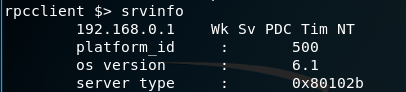
\includegraphics{/rpcclient/srvinfo.PNG}
	\section{RPCClient QueryDomInfo}
		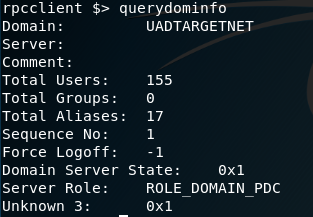
\includegraphics{/rpcclient/querydominfo.PNG}
	\section{RPCClient EnumDomUsers}
		\begin{lstlisting}
user:[Administrator] rid:[0x1f4]
user:[Guest] rid:[0x1f5]
user:[krbtgt] rid:[0x1f6]
user:[Benny Hill] rid:[0x3e8]
user:[R.Gudino] rid:[0x20da]
user:[E.Breck] rid:[0x20db]
user:[D.Lecroy] rid:[0x20dc]
user:[C.Armes] rid:[0x20dd]
user:[C.Yother] rid:[0x20de]
user:[K.Dipaola] rid:[0x20df]
user:[M.Lanasa] rid:[0x20e0]
user:[D.Clinard] rid:[0x20e1]
user:[W.Parekh] rid:[0x20e2]
user:[N.Hooton] rid:[0x20e3]
user:[D.Mcdonough] rid:[0x20e4]
user:[M.Bonneau] rid:[0x20e5]
user:[F.Nelms] rid:[0x20e6]
user:[E.Hillhouse] rid:[0x20e7]
user:[M.Lampe] rid:[0x20e8]
user:[L.Mcnaughton] rid:[0x20e9]
user:[D.Halas] rid:[0x20ea]
user:[R.Burstein] rid:[0x20eb]
user:[V.Layman] rid:[0x20ec]
user:[A.Marsland] rid:[0x20ed]
user:[D.Rosamond] rid:[0x20ee]
user:[B.Riche] rid:[0x20ef]
user:[J.Wiste] rid:[0x20f0]
user:[T.Lefebre] rid:[0x20f1]
user:[S.Dalrymple] rid:[0x20f2]
user:[R.Stoneking] rid:[0x20f3]
user:[S.Russom] rid:[0x20f4]
user:[M.Maxwell] rid:[0x20f5]
user:[Z.Sowders] rid:[0x20f6]
user:[M.Hoy] rid:[0x20f7]
user:[C.Selzer] rid:[0x20f8]
user:[K.Leiker] rid:[0x20f9]
user:[S.Gerst] rid:[0x20fa]
user:[D.Kennemer] rid:[0x20fb]
user:[L.Angelo] rid:[0x20fc]
user:[L.Gamino] rid:[0x20fd]
user:[S.Tacey] rid:[0x20fe]
user:[E.Bouknight] rid:[0x20ff]
user:[L.Soriano] rid:[0x2100]
user:[M.Wentz] rid:[0x2101]
user:[G.Fuller] rid:[0x2102]
user:[C.Linen] rid:[0x2103]
user:[J.Murrell] rid:[0x2104]
user:[A.Eisenmenger] rid:[0x2105]
user:[S.Poore] rid:[0x2106]
user:[A.Fritzler] rid:[0x2107]
user:[M.Otter] rid:[0x2108]
user:[S.Kerfoot] rid:[0x2109]
user:[B.Saari] rid:[0x210a]
user:[M.Colberg] rid:[0x210b]
user:[V.Reighard] rid:[0x210c]
user:[S.Leverich] rid:[0x210d]
user:[C.Hernadez] rid:[0x210e]
user:[E.Bolander] rid:[0x210f]
user:[S.Abercrombie] rid:[0x2110]
user:[D.Kawasaki] rid:[0x2111]
user:[J.Killion] rid:[0x2112]
user:[C.Spann] rid:[0x2113]
user:[E.Bascom] rid:[0x2114]
user:[W.Haakenson] rid:[0x2115]
user:[K.Corney] rid:[0x2116]
user:[K.Husby] rid:[0x2117]
user:[R.Avina] rid:[0x2118]
user:[C.Corpuz] rid:[0x2119]
user:[M.Tilman] rid:[0x211a]
user:[T.Blass] rid:[0x211b]
user:[B.Schweitzer] rid:[0x211c]
user:[W.Loch] rid:[0x211d]
user:[N.Broady] rid:[0x211e]
user:[L.Sarver] rid:[0x211f]
user:[F.Ousley] rid:[0x2120]
user:[T.Prestidge] rid:[0x2121]
user:[G.Nordeen] rid:[0x2122]
user:[G.Youngberg] rid:[0x2123]
user:[R.Zoll] rid:[0x2124]
user:[M.Thiel] rid:[0x2125]
user:[N.Bitterman] rid:[0x2126]
user:[V.Teran] rid:[0x2127]
user:[M.Pascucci] rid:[0x2128]
user:[F.Lu] rid:[0x2129]
user:[I.Cortright] rid:[0x212a]
user:[M.Birdwell] rid:[0x212b]
user:[E.Mogan] rid:[0x212c]
user:[F.Lietz] rid:[0x212d]
user:[A.Mckendree] rid:[0x212e]
user:[R.Sepeda] rid:[0x212f]
user:[D.Doolin] rid:[0x2130]
user:[J.Schack] rid:[0x2131]
user:[E.Leclaire] rid:[0x2132]
user:[J.Uribe] rid:[0x2133]
user:[Y.Lezama] rid:[0x2134]
user:[B.Evert] rid:[0x2135]
user:[D.Jin] rid:[0x2136]
user:[O.Sandoval] rid:[0x2137]
user:[Y.Weinstein] rid:[0x2138]
user:[C.Brice] rid:[0x2139]
user:[H.Shiba] rid:[0x213a]
user:[G.Chica] rid:[0x213b]
user:[M.Hershberger] rid:[0x213c]
user:[test] rid:[0x213e]
		\end{lstlisting}
	\section{RPCClient LookupNames Administrators}
		
\includegraphics{/rpcclient/lookupnames_administrators.PNG}
	\section{RPCClient LookupNames Administrator}
		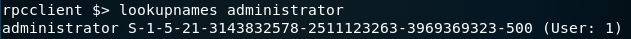
\includegraphics{/rpcclient/lookupnames_administrator.PNG}
	\section{NetBIOS Command Console}
		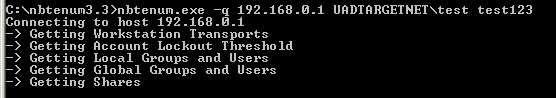
\includegraphics{/nbtenum/nbtenum.PNG}
	\section{NetBIOS Admin List}
		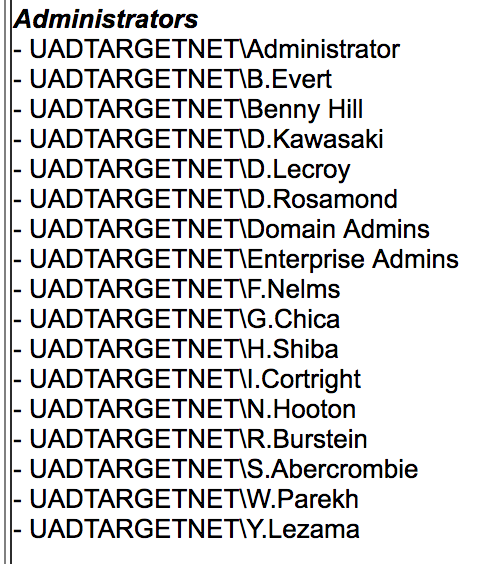
\includegraphics{/nbtenum/admins.png}
	\section{Nessus Server 1 Output}
		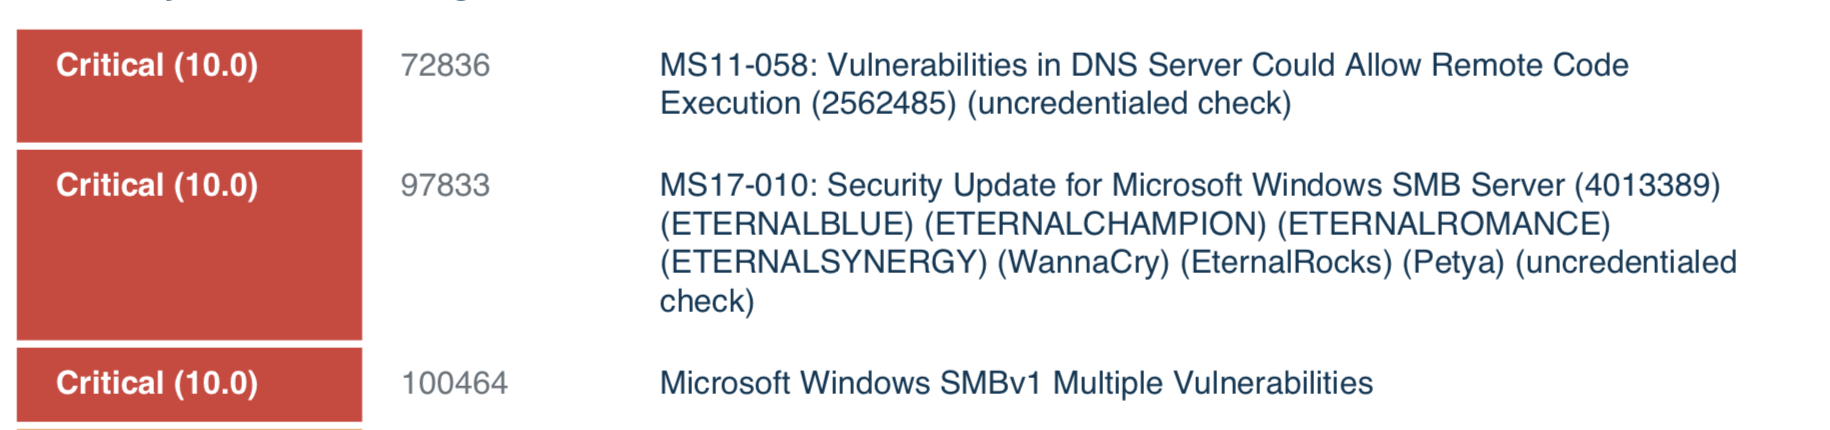
\includegraphics[scale=0.5]{/nessus/server1.png}
	\section{Nessus Client 1 Output}
		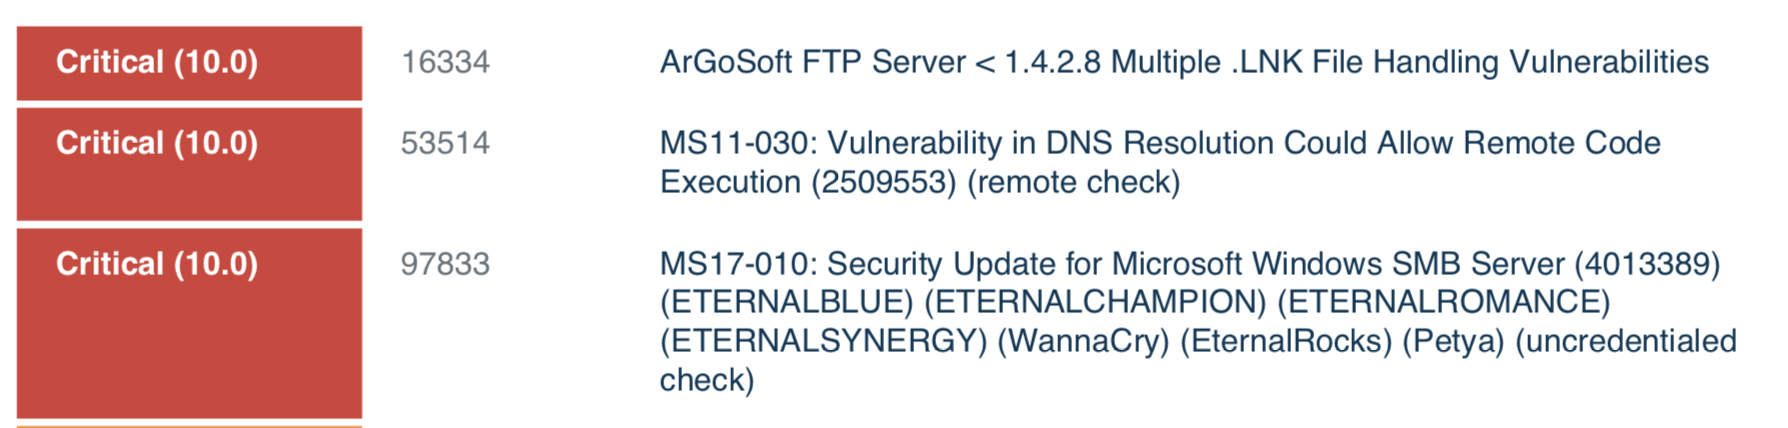
\includegraphics[scale=0.5]{/nessus/client1.png}
	\section{Metasploit Setting Payload}
		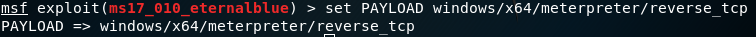
\includegraphics[scale=0.75]{/meterpreter/setting_payload.PNG}
	\section{Metasploit Setting Remote Host}
		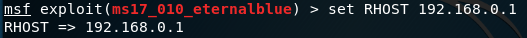
\includegraphics{/meterpreter/setting_rhost.PNG}
	\section{Metasploit Setting Local Host}
		
\includegraphics{/meterpreter/setting_lhost.PNG}
	\section{Metasploit Re-setting Remote Host}
		
\includegraphics{/meterpreter/server2_LHOST.PNG}
	\section{Metasploit Hash Dump}
		\begin{lstlisting}
Administrator:500:aad3b435b51404eeaad3b435b51404ee:e53c09abd08dbd99c43a1efec560f45f:::
Guest:501:aad3b435b51404eeaad3b435b51404ee:31d6cfe0d16ae931b73c59d7e0c089c0:::
krbtgt:502:aad3b435b51404eeaad3b435b51404ee:ab4f1664ad3a8ac47a90d02b3cc4fa37:::
Benny Hill:1000:aad3b435b51404eeaad3b435b51404ee:8516f8dca38b8541bc6f4732c3b304f2:::
R.Gudino:8410:aad3b435b51404eeaad3b435b51404ee:a16cd1df23cf8b8e923b312e9ab3f5d4:::
E.Breck:8411:aad3b435b51404eeaad3b435b51404ee:483ec4b04b0a552316b276c2624a34fa:::
D.Lecroy:8412:aad3b435b51404eeaad3b435b51404ee:c53064e9887a83f8a4d5cbfcef972305:::
C.Armes:8413:aad3b435b51404eeaad3b435b51404ee:854b0771463f88f7bc24a4725f84e8cb:::
C.Yother:8414:aad3b435b51404eeaad3b435b51404ee:676035f793cc21d58a224011ea06bab2:::
K.Dipaola:8415:aad3b435b51404eeaad3b435b51404ee:97bab9d5bece0fcc4f1e4276b86b7cd2:::
M.Lanasa:8416:aad3b435b51404eeaad3b435b51404ee:6b9e4e4fe9908b12391c41ef35b7b1c3:::
D.Clinard:8417:aad3b435b51404eeaad3b435b51404ee:81fdfb48450ad4f3864d741a01ca2e21:::
W.Parekh:8418:aad3b435b51404eeaad3b435b51404ee:24e4ac391f7c5d4378f792253e356f22:::
N.Hooton:8419:aad3b435b51404eeaad3b435b51404ee:a6339833fd0bcf84a3ab10a42fa7b59a:::
D.Mcdonough:8420:aad3b435b51404eeaad3b435b51404ee:ce1dc95c9d025db2e1f3ea85c40236be:::
M.Bonneau:8421:aad3b435b51404eeaad3b435b51404ee:c8772704bdf47b48a33804df97f67850:::
F.Nelms:8422:aad3b435b51404eeaad3b435b51404ee:f64237b0e85352bd41ce8eed475d8421:::
E.Hillhouse:8423:aad3b435b51404eeaad3b435b51404ee:f62a557ef50f7784877e4f9a56e159e6:::
M.Lampe:8424:aad3b435b51404eeaad3b435b51404ee:d8d5907791e5a47726e83e5e46f2af40:::
L.Mcnaughton:8425:aad3b435b51404eeaad3b435b51404ee:24b5431395c05f8b51ea696b56a753d5:::
D.Halas:8426:aad3b435b51404eeaad3b435b51404ee:4096de2eb2481c54b9434504a6bd2626:::
R.Burstein:8427:aad3b435b51404eeaad3b435b51404ee:dbd5e86f519091ee6bd8493ab5a11495:::
V.Layman:8428:aad3b435b51404eeaad3b435b51404ee:43bcce94858487616e05d95296ede293:::
A.Marsland:8429:aad3b435b51404eeaad3b435b51404ee:73e649125bc403926b144d55afb39b93:::
D.Rosamond:8430:aad3b435b51404eeaad3b435b51404ee:70e0448c608d9a2c9063f843a67e19ea:::
B.Riche:8431:aad3b435b51404eeaad3b435b51404ee:889f1e1dda555e1dbf1dd2fddeab883d:::
J.Wiste:8432:aad3b435b51404eeaad3b435b51404ee:bd2ec47441828680d9e0505cf0459e5c:::
T.Lefebre:8433:aad3b435b51404eeaad3b435b51404ee:4b4e6698bfe9dc66f21fccee2b3a716f:::
S.Dalrymple:8434:aad3b435b51404eeaad3b435b51404ee:0e22d6c69b26a876faae86c723e905fc:::
R.Stoneking:8435:aad3b435b51404eeaad3b435b51404ee:68ca4d1dd6450dee4940a9bcb4ce8423:::
S.Russom:8436:aad3b435b51404eeaad3b435b51404ee:3ef78cda39b74b1c181814af284fb3f1:::
M.Maxwell:8437:aad3b435b51404eeaad3b435b51404ee:840a1f2263dd7dffdf4d0ac22dcc6f49:::
Z.Sowders:8438:aad3b435b51404eeaad3b435b51404ee:8519eb53ce4e373f984a0e38f4b810fb:::
M.Hoy:8439:aad3b435b51404eeaad3b435b51404ee:a7b07e7189039642f865bb96a9c35570:::
C.Selzer:8440:aad3b435b51404eeaad3b435b51404ee:d275a92aeef9d6b958d22dd34e2d33cb:::
K.Leiker:8441:aad3b435b51404eeaad3b435b51404ee:9ca781b2c9b0e2db50ac628846f852f5:::
S.Gerst:8442:aad3b435b51404eeaad3b435b51404ee:a2eb2c7035aaf261e099a4f345f14980:::
D.Kennemer:8443:aad3b435b51404eeaad3b435b51404ee:bba45f0275135400fe21015d52d937b1:::
L.Angelo:8444:aad3b435b51404eeaad3b435b51404ee:c4342458001cd63d599b200ad74cb09e:::
L.Gamino:8445:aad3b435b51404eeaad3b435b51404ee:eb48f0585453625ec4e4ed116977042e:::
S.Tacey:8446:aad3b435b51404eeaad3b435b51404ee:edccee80b5097606b5e1a991ff20d0ab:::
E.Bouknight:8447:aad3b435b51404eeaad3b435b51404ee:53124ae8313a8f4b6e28eec9b978e41c:::
L.Soriano:8448:aad3b435b51404eeaad3b435b51404ee:fede29a42ffcb3cf0955d8f7ca567955:::
M.Wentz:8449:aad3b435b51404eeaad3b435b51404ee:9568d16ab2ccf3f4801678eda8bc749d:::
G.Fuller:8450:aad3b435b51404eeaad3b435b51404ee:e65f96ff47fbb707c4af42aced95d43b:::
C.Linen:8451:aad3b435b51404eeaad3b435b51404ee:99b6dd12c417c650d1f968b8afdde36e:::
J.Murrell:8452:aad3b435b51404eeaad3b435b51404ee:3fabd7fc9b1a83b16370168f7fbc741e:::
A.Eisenmenger:8453:aad3b435b51404eeaad3b435b51404ee:583018f6618d5cb7004b6af75eadf510:::
S.Poore:8454:aad3b435b51404eeaad3b435b51404ee:2ece90083724c6050f1d7d54b57c13e0:::
A.Fritzler:8455:aad3b435b51404eeaad3b435b51404ee:6ac6a6fd88899f637cde5f2e6564a1e1:::
M.Otter:8456:aad3b435b51404eeaad3b435b51404ee:86439a616978705185f584bf350cf5dc:::
S.Kerfoot:8457:aad3b435b51404eeaad3b435b51404ee:8cb3522398cbe3dbd0abe6a26a87478e:::
B.Saari:8458:aad3b435b51404eeaad3b435b51404ee:53b1fd8b95ec2299731c623d948276c6:::
M.Colberg:8459:aad3b435b51404eeaad3b435b51404ee:1ac6ed1b576eb48ddf6676d0bb2aa3e5:::
V.Reighard:8460:aad3b435b51404eeaad3b435b51404ee:467e2d0e0e8daaf270d82b9dcc7124c6:::
S.Leverich:8461:aad3b435b51404eeaad3b435b51404ee:b5b73b1984e9c951d4e95924a1cbc34f:::
C.Hernadez:8462:aad3b435b51404eeaad3b435b51404ee:e4e95bee1e9e9b4d49020c3b659d85f3:::
E.Bolander:8463:aad3b435b51404eeaad3b435b51404ee:c6504719856851983a0ccc47f009ae96:::
S.Abercrombie:8464:aad3b435b51404eeaad3b435b51404ee:5375fdb80376829e2a30271aa81640c1:::
D.Kawasaki:8465:aad3b435b51404eeaad3b435b51404ee:08d8ed1eaeea3c8fd7acc06314976e36:::
J.Killion:8466:aad3b435b51404eeaad3b435b51404ee:6117435384806d5c98df5c4e3d0ae712:::
C.Spann:8467:aad3b435b51404eeaad3b435b51404ee:8d4aed79e85b97d730a06b0bea01a085:::
E.Bascom:8468:aad3b435b51404eeaad3b435b51404ee:1f4ad2c305a1624d9e53bf1c34ad6977:::
W.Haakenson:8469:aad3b435b51404eeaad3b435b51404ee:2cbec3d1df634a653b2b2a07e411a11a:::
K.Corney:8470:aad3b435b51404eeaad3b435b51404ee:071650fb910bcf433f0944c2a48234f5:::
K.Husby:8471:aad3b435b51404eeaad3b435b51404ee:9ba3b63f93788a77e9cd5ae290e35f9c:::
R.Avina:8472:aad3b435b51404eeaad3b435b51404ee:280635941483e80a3ba540cae061754d:::
C.Corpuz:8473:aad3b435b51404eeaad3b435b51404ee:c18f63bfcf49f049c9a4ea12fa5150b7:::
M.Tilman:8474:aad3b435b51404eeaad3b435b51404ee:47b55ceed18efe45582bab180dcc6ce3:::
T.Blass:8475:aad3b435b51404eeaad3b435b51404ee:8b121c8bc35ba87546985582f3329b8d:::
B.Schweitzer:8476:aad3b435b51404eeaad3b435b51404ee:00860eb7c07bd00e9945faa01877b89a:::
W.Loch:8477:aad3b435b51404eeaad3b435b51404ee:90584e3a0a419f3e208da1b39b2ec98a:::
N.Broady:8478:aad3b435b51404eeaad3b435b51404ee:ce055cd6aca06cb629bce80c7bcae5d2:::
L.Sarver:8479:aad3b435b51404eeaad3b435b51404ee:bf99adbdc97c1f9a1ad9f4efc4dd4be3:::
F.Ousley:8480:aad3b435b51404eeaad3b435b51404ee:53effa66137a652ea07b6a6b8451ac6e:::
T.Prestidge:8481:aad3b435b51404eeaad3b435b51404ee:f7d460e1c769b6a8a68ca878cfedf5ce:::
G.Nordeen:8482:aad3b435b51404eeaad3b435b51404ee:05a3d4704d52997e255c4dc0ba3fae1c:::
G.Youngberg:8483:aad3b435b51404eeaad3b435b51404ee:e1f0f84ff05796020ef43891709cfc77:::
R.Zoll:8484:aad3b435b51404eeaad3b435b51404ee:129e6028e32aac47d9fd5bfc91be3911:::
M.Thiel:8485:aad3b435b51404eeaad3b435b51404ee:17ad717e4fb4ee6f547a72b64bdc3c75:::
N.Bitterman:8486:aad3b435b51404eeaad3b435b51404ee:fcc3b78f9abf782da2ba68d9bc6902f5:::
V.Teran:8487:aad3b435b51404eeaad3b435b51404ee:af0e992f816167feebe71d57db83e0c2:::
M.Pascucci:8488:aad3b435b51404eeaad3b435b51404ee:a010c0cf64975ce361e428b701b15c91:::
F.Lu:8489:aad3b435b51404eeaad3b435b51404ee:b6e4332e1cebf538eb367127203c71ba:::
I.Cortright:8490:aad3b435b51404eeaad3b435b51404ee:9c12c32215cdf257506d6623c676a4e5:::
M.Birdwell:8491:aad3b435b51404eeaad3b435b51404ee:d6795acdd456261a959f67837d28886a:::
E.Mogan:8492:aad3b435b51404eeaad3b435b51404ee:79e84653d30fe67c7b5ae45eb3c6eb48:::
F.Lietz:8493:aad3b435b51404eeaad3b435b51404ee:6dd01db8c84aa3ae833f1c4cce0d7f98:::
A.Mckendree:8494:aad3b435b51404eeaad3b435b51404ee:8307c7288138647ab7691e1674819b63:::
R.Sepeda:8495:aad3b435b51404eeaad3b435b51404ee:12a1e6d68055762e2d8fc61d9215b3ee:::
D.Doolin:8496:aad3b435b51404eeaad3b435b51404ee:3a1b01992f7f12d79d1775148bac1775:::
J.Schack:8497:aad3b435b51404eeaad3b435b51404ee:6ea9ce1a4aeb73e7ddd4a194a4dbafd2:::
E.Leclaire:8498:aad3b435b51404eeaad3b435b51404ee:d4a39cccec6bcff8acec23b572a2dd9e:::
J.Uribe:8499:aad3b435b51404eeaad3b435b51404ee:38cf160ebc6020e49a91f9a0472a281a:::
Y.Lezama:8500:aad3b435b51404eeaad3b435b51404ee:34486d10c832e47a9ae1e5af73cdfc19:::
B.Evert:8501:aad3b435b51404eeaad3b435b51404ee:9b8d4df3379439d96bcc45426f70f9d2:::
D.Jin:8502:aad3b435b51404eeaad3b435b51404ee:668a80793e5bef2b6aaee72e00d59355:::
O.Sandoval:8503:aad3b435b51404eeaad3b435b51404ee:1db8c250285adcfdb68169bfacf09119:::
Y.Weinstein:8504:aad3b435b51404eeaad3b435b51404ee:e761047004fe0282a9222b27784fd8de:::
C.Brice:8505:aad3b435b51404eeaad3b435b51404ee:b719beb7f6d7473e4f5ee57687b9b7e5:::
H.Shiba:8506:aad3b435b51404eeaad3b435b51404ee:1348eb6f945ebb332f6d69a3b8f4f7c1:::
G.Chica:8507:aad3b435b51404eeaad3b435b51404ee:062c72bc7417f9bafdaf0625003435f2:::
M.Hershberger:8508:aad3b435b51404eeaad3b435b51404ee:43efd4b4078817357c3bafed63f13dd9:::
test:8510:aad3b435b51404eeaad3b435b51404ee:c5a237b7e9d8e708d8436b6148a25fa1:::
SERVER1$:1001:aad3b435b51404eeaad3b435b51404ee:9683fcd45319937ac8d7d4428e94f6d5:::
webs$:8511:aad3b435b51404eeaad3b435b51404ee:1da4fffcb02780085b145e024f93c930:::
secured$:8512:aad3b435b51404eeaad3b435b51404ee:e7bc7fe66d393afd0517d7ea0e9e6667:::
lists$:8513:aad3b435b51404eeaad3b435b51404ee:9af17b2c7237b550b708b54f9d40b8a1:::
pc56$:8514:aad3b435b51404eeaad3b435b51404ee:4f355eaad5550fdaecaded16ca0b02ea:::
rtc5$:8515:aad3b435b51404eeaad3b435b51404ee:f9fd69e581463b17abae5ffc60a2a428:::
cn$:8516:aad3b435b51404eeaad3b435b51404ee:f99a805dc0e1a52b597537a35bf84545:::
wwwchat$:8517:aad3b435b51404eeaad3b435b51404ee:5b43dc6031b23170af3e403ebe26351e:::
lib$:8518:aad3b435b51404eeaad3b435b51404ee:7d341633c2d9f03f9868d83936b174f2:::
pc54$:8519:aad3b435b51404eeaad3b435b51404ee:10e68484cd5a756ebe842facac09047e:::
rho$:8520:aad3b435b51404eeaad3b435b51404ee:39309d445a248bc196009eedfac78059:::
cust21$:8521:aad3b435b51404eeaad3b435b51404ee:18cafb825f99a30ce7b727734a1ec416:::
cust39$:8522:aad3b435b51404eeaad3b435b51404ee:43425fa99705f9e156267c9c0f5cef47:::
ipmonitor$:8523:aad3b435b51404eeaad3b435b51404ee:0cf53cba9583f8d6cffdcf6c276864b3:::
galerias$:8524:aad3b435b51404eeaad3b435b51404ee:7cd3f768f390193d20fc30102a886f65:::
segment-119-227$:8525:aad3b435b51404eeaad3b435b51404ee:33e9c2af25801b2928b025b24a3a1138:::
b$:8526:aad3b435b51404eeaad3b435b51404ee:93e6524fb0368bf63d2d6a3674c210ab:::
pc19$:8527:aad3b435b51404eeaad3b435b51404ee:d830437fb15a8a8fa3080613eaadbefe:::
correo$:8528:aad3b435b51404eeaad3b435b51404ee:63b4b3fc4a00ecbed8a2ed9d35072a86:::
uranus$:8529:aad3b435b51404eeaad3b435b51404ee:37214569b4edec77af0b8edeb18342c2:::
miami$:8530:aad3b435b51404eeaad3b435b51404ee:e920b255bb70cd9194c15055f7925155:::
CLIENT1$:8532:aad3b435b51404eeaad3b435b51404ee:28e72742632fa1f371d2885a12e69a95:::
CLIENT2$:8533:aad3b435b51404eeaad3b435b51404ee:49b813d6970c12e83e3a8f927d81ea1a:::
SERVER2$:8534:aad3b435b51404eeaad3b435b51404ee:987e2eb29c51ab1b58cbee8392ca8321:::
		\end{lstlisting}
	\section{Using Cain to Crack the Hashes}
		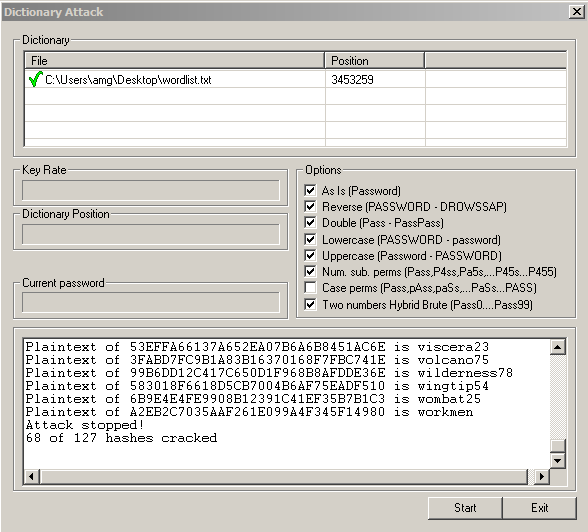
\includegraphics{/cain/caincrack.PNG}
	\section{Cracked Administrator Account}
		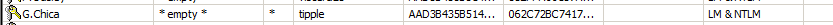
\includegraphics[scale=0.75]{/cain/hchica.PNG}
	\section{Logged in with Administrative Privileges}
		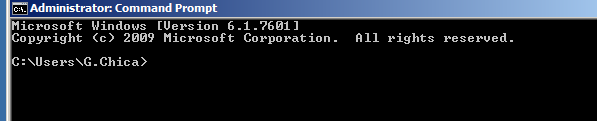
\includegraphics{/penetration/admin_console.PNG}
	\section{Hydra Input}
		
\includegraphics[scale=0.75]{/hydra/hydra.PNG}
	\section{Hydra Output}
		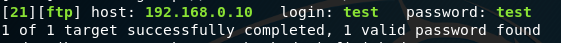
\includegraphics[scale=0.5]{/hydra/hydra_success.PNG}

	\end{appendices}

%% -- END OF DOCUMENT -- %%
\end{document}

											%% - 0 - %%
